\documentclass[11pt,a4paper]{article}
\usepackage[a4paper,margin=2.4cm]{geometry}
\usepackage{amsmath}
\usepackage{enumitem}
\usepackage{graphicx}
\usepackage{booktabs}
\usepackage{pgfplots}
\pgfplotsset{compat=1.18}
\definecolor{rider}{HTML}{1D5BBF}
\definecolor{driver}{HTML}{A8520A}
\definecolor{ridersoft}{HTML}{DCE7F8}
\definecolor{driversoft}{HTML}{F6E5D3}
\definecolor{quiet}{HTML}{A3AAB8}

% one matched pair as a bar split into the rider's share and the driver's share
\newcommand{\splitbar}[4]{%
  \fill[rider] (0,#1) rectangle (#2*0.36,#1+0.42);
  \fill[driver] (#2*0.36,#1) rectangle (#2*0.36+#3*0.36,#1+0.42);
  \ifdim #2pt>0pt \node[white,font=\scriptsize\bfseries,anchor=west] at (0.02,#1+0.21) {#2};\fi
  \ifdim #3pt>0pt \node[white,font=\scriptsize\bfseries,anchor=east] at (#2*0.36+#3*0.36-0.02,#1+0.21) {#3};\fi
  \node[font=\scriptsize,anchor=east] at (-0.1,#1+0.21) {#4};}
\setlist[itemize]{itemsep=2pt,topsep=3pt}
\setlength{\abovecaptionskip}{4pt}

\title{\textbf{Core Pricing in Learned Assignment Markets}}
\author{Anirudh Jain \and Ayush Pandey \and Sourabh}
\date{}

\begin{document}
\vspace{-2em}
\maketitle
\vspace{-1.5em}

\begin{quote}
\textbf{When a ride-hailing platform matches riders to drivers using predicted (noisy) surplus values, how much do the optimal matching and the stable (core) prices change with prediction error, can riders or drivers gain by misreporting, and which stable price should the platform choose?}
\end{quote}

A ride-hailing platform makes two decisions: which rider rides with which driver, and how the value of each trip is split between them. Both come from one linear program. The matching is an assignment LP, and the split comes from its dual. The platform does not know the true values of each trip; it predicts them, and predictions are wrong by some amount. This project measures what those errors do to the matching and to the prices, checks whether a rider or driver can gain by lying about their values, and uses a small game to choose the safest price.

\section{The Core: Matching, Prices and Stability}

\textbf{Setup.} For rider $i$ and driver $j$, the surplus $a_{ij}\ge0$ is what the rider would pay for the trip minus what it costs the driver: the value the pair creates together. The platform sees only a prediction of it. We write a prediction as the true surplus plus a random error, $\hat a_{ij}=\max(a_{ij}+\varepsilon_{ij},0)$ with $\varepsilon_{ij}\sim N(0,\sigma^2)$, where $\sigma$ is how inaccurate the predictor is. Any prediction method can be written as truth plus error, so varying $\sigma$ covers good and bad predictors alike.

\textbf{Matching.} With $x_{ij}=1$ when rider $i$ rides with driver $j$, the platform solves
\[
V=\max \sum_{i,j} a_{ij}x_{ij}
\quad\text{s.t.}\quad
\sum_j x_{ij}\le 1\;\;(\text{rider } i),\qquad \sum_i x_{ij}\le 1\;\;(\text{driver } j),\qquad x\ge 0 .
\]
This is the assignment problem. Its constraint matrix is totally unimodular, so the simplex optimum is already 0 or 1.

\textbf{Prices.} The dual LP is
\[
\min \sum_i u_i+\sum_j v_j
\quad\text{s.t.}\quad
u_i+v_j\ge a_{ij},\qquad u,v\ge 0 .
\]
We read $u_i$ as the part of the surplus that rider $i$ keeps and $v_j$ as the part driver $j$ keeps; together they fix the fare. The constraint $u_i+v_j\ge a_{ij}$ says that no rider and driver can both do better by leaving the platform and splitting $a_{ij}$ on their own. A pair with $u_i+v_j<a_{ij}$ would leave; we say it \emph{blocks}. Prices with no blocking pair that pay out exactly $V$ form the \emph{core}, and Shapley and Shubik~\cite{shapley} proved that the core is exactly the set of optimal dual solutions. By complementary slackness a matched pair splits exactly its own surplus, and an unmatched person gets 0.

\textbf{Three price points.} The dual has many optimal solutions, so the core is a range of prices for the same matching. Its two ends are easy to compute. At the rider-optimal point (RO) each rider gets their marginal contribution $u_i=V-V_{-i}$, where $V_{-i}$ is the best total without rider $i$, and each matched driver gets the rest, $v_j=a_{ij}-u_i$. The driver-optimal point (DO) does the same for drivers. MID is the average of the two, and any mix of RO and DO is again in the core.

\textbf{Example.} We use two small markets. $A=\begin{pmatrix}10&6\\7&4\end{pmatrix}$ has $V=14$, RO $u=(7,4)$, $v=(3,0)$ and DO $u=(2,0)$, $v=(8,4)$. The main market $B$ has three riders and three drivers:
\[
B=\begin{pmatrix}12&10&6\\11&7&4\\9&11&9\end{pmatrix},\qquad V=30,\quad \text{matching } R1\text{--}D2,\; R2\text{--}D1,\; R3\text{--}D3 .
\]
The next best matching is worth 28. Table~\ref{tab:core} and Figures~\ref{fig:split} and~\ref{fig:ranges} give the prices. Every share can move by 7, and the riders' total goes from 3 at DO to 24 at RO: 21 of the 30 units change sides while the matching stays the same. The choice of price point decides who gets the surplus.

\begin{table}[h]
\centering\small
\begin{tabular}{lccccccc}
\toprule
Point & $u_1$ & $u_2$ & $u_3$ & $v_1$ & $v_2$ & $v_3$ & $\sum u$ \\
\midrule
RO  & 8   & 7   & 9   & 4   & 2   & 0   & 24 \\
MID & 4.5 & 3.5 & 5.5 & 7.5 & 5.5 & 3.5 & 13.5 \\
DO  & 1   & 0   & 2   & 11  & 9   & 7   & 3 \\
\bottomrule
\end{tabular}
\caption{The three price points of $B$. Each row sums to $V=30$ and has no blocking pair.}
\label{tab:core}
\end{table}

\begin{figure}[htbp]
\centering
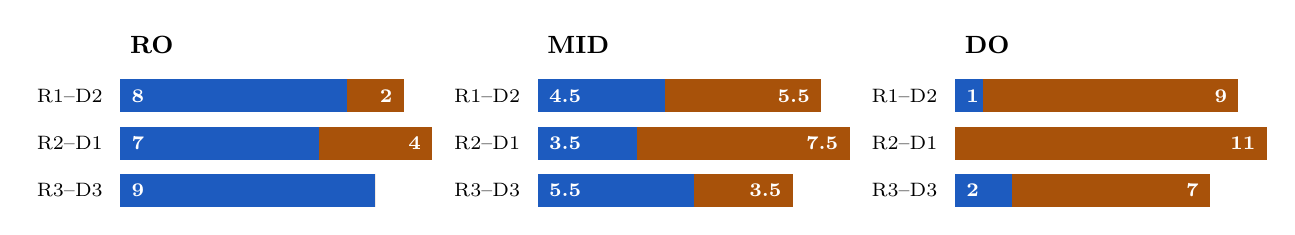
\begin{tikzpicture}
\foreach \name/\x/\a/\b/\c/\d/\e/\f in {RO/0/8/2/7/4/9/0, MID/5.3/4.5/5.5/3.5/7.5/5.5/3.5, DO/10.6/1/9/0/11/2/7} {
  \begin{scope}[xshift=\x cm]
    \node[font=\small\bfseries,anchor=west] at (0,2.05) {\name};
    \splitbar{1.2}{\a}{\b}{R1--D2}
    \splitbar{0.6}{\c}{\d}{R2--D1}
    \splitbar{0}{\e}{\f}{R3--D3}
  \end{scope}
}
\end{tikzpicture}
\caption{How each matched pair of $B$ splits its surplus at the three price points: rider's share in blue, driver's share in amber. The pairs stay the same; only the split moves.}
\label{fig:split}
\end{figure}

\begin{figure}[h]
\centering
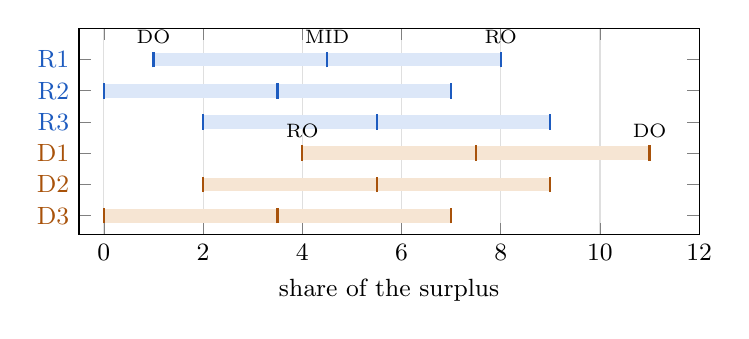
\begin{tikzpicture}
\begin{axis}[
  width=0.78\textwidth, height=4.2cm,
  xmin=-0.5, xmax=12, ymin=0.4, ymax=7,
  ytick={1,...,6}, yticklabels={\textcolor{driver}{D3},\textcolor{driver}{D2},\textcolor{driver}{D1},\textcolor{rider}{R3},\textcolor{rider}{R2},\textcolor{rider}{R1}},
  xlabel={share of the surplus}, xtick={0,2,...,12},
  xmajorgrids, grid style={gray!25}, tick label style={font=\small}, label style={font=\small}]
\foreach \y/\lo/\mid/\hi/\c in {6/1/4.5/8/rider, 5/0/3.5/7/rider, 4/2/5.5/9/rider, 3/4/7.5/11/driver, 2/2/5.5/9/driver, 1/0/3.5/7/driver} {
  \edef\temp{\noexpand\draw[line width=5pt, \c soft] (axis cs:\lo,\y) -- (axis cs:\hi,\y);
    \noexpand\draw[thick, \c] (axis cs:\lo,\y-0.25) -- (axis cs:\lo,\y+0.25);
    \noexpand\draw[thick, \c] (axis cs:\hi,\y-0.25) -- (axis cs:\hi,\y+0.25);
    \noexpand\draw[thick, \c] (axis cs:\mid,\y-0.25) -- (axis cs:\mid,\y+0.25);}
  \temp
}
\node[font=\scriptsize, above] at (axis cs:8,6.2) {RO};
\node[font=\scriptsize, above] at (axis cs:1,6.2) {DO};
\node[font=\scriptsize, above] at (axis cs:4.5,6.2) {MID};
\node[font=\scriptsize, above] at (axis cs:4,3.2) {RO};
\node[font=\scriptsize, above] at (axis cs:11,3.2) {DO};
\end{axis}
\end{tikzpicture}
\caption{The range of stable shares for each rider (blue) and driver (amber) in $B$. A rider's share is lowest at DO and highest at RO; a driver's is the other way round. The middle tick is MID.}
\label{fig:ranges}
\end{figure}

\textbf{Sensitivity analysis.} Change rider $i$'s right-hand side from 1 to $b$. The best total $V(b)$ is piecewise linear in $b$; at $b=1$ its slope from the left is rider $i$'s largest core share and its slope from the right the smallest. For rider 1 of $B$ these are $30-22=8$ and 1, the two ends of its range. A simplex solver prints only one shadow price. Because the optimal basis is degenerate (a basic variable equals 0), that price has an allowable increase or decrease of 0 on one side. That zero is the core range seen through sensitivity analysis, and TORA shows it (Section~2).

\textbf{Hungarian method.} Maximising $a$ is the same as minimising $12-a$. Row reduction, column reduction and one adjustment (two lines cover all zeros, fewer than 3, so subtract the smallest uncovered entry, 2) give
\[
\begin{pmatrix}0&2&6\\1&5&8\\3&1&3\end{pmatrix}\!\to\!
\begin{pmatrix}0&2&6\\0&4&7\\2&0&2\end{pmatrix}\!\to\!
\begin{pmatrix}0&2&4\\0&4&5\\2&0&0\end{pmatrix}\!\to\!
\begin{pmatrix}0&\mathbf{0}&2\\\mathbf{0}&2&3\\4&0&\mathbf{0}\end{pmatrix}.
\]
The bold zeros give R1--D2, R2--D1, R3--D3 at cost $36-30=6$, the same matching as the LP.

\textbf{Syllabus topics used.} LP formulation and the simplex method (the assignment LP; the RO and DO LPs need the M-method for their $\ge$ and $=$ constraints), duality and sensitivity (prices are the dual solution; a price range is a degenerate shadow price), the transportation and assignment problems (northwest corner, least cost, Vogel and the Hungarian method), and game theory (saddle points, the graphical method and a game solved as an LP).

\section{Relationship to TORA: Hand Solutions and Code}

Every model small enough to type in was solved in TORA~\cite{taha} and compared with our code:
\begin{itemize}
  \item the assignment LP for $A$ (4 variables, 4 constraints) and $B$ (9 variables, 6 constraints), with dual prices and sensitivity analysis;
  \item the RO and DO LPs: maximise or minimise $\sum u_i$ subject to $u_i+v_j\ge a_{ij}$ and $\sum u+\sum v=V$, by the M-method;
  \item the assignment as a transportation problem, with every supply and demand equal to 1 and cost $12-a$ for $B$ ($10-a$ for $A$), from northwest corner, least cost and Vogel starts;
  \item the pricing game of Section~3.3 as an LP.
\end{itemize}
Every value agrees (Table~\ref{tab:tora}, Figure~\ref{fig:tora}). Three outputs say more than the totals:
\begin{itemize}
  \item For $A$, TORA's dual prices are $(7,4)$ for the riders and $(3,0)$ for the drivers, which is the RO point. Its RHS ranges show the degeneracy: the rider rows cannot increase (maximum RHS 1) and the driver rows cannot decrease (minimum RHS 1).
  \item In the transportation model of $B$, the northwest corner start costs 8 and needs one iteration to reach 6, while Vogel's start is already optimal. Both end on the LP's matching, with zero cells in the basis, the same degeneracy.
  \item The game LP gives $w=2$ (value 1) and $p=(0.5,0,0.5)$, and reports alternative optima because pure MID is also optimal. Its dual prices on the two payoff rows are 0.5 and 0.5 (printed as $-0.5$ for a minimisation), which is the manipulator's best mix. One LP solves both players.
\end{itemize}

\begin{table}[h]
\centering\small
\begin{tabular}{lcc@{\hspace{2.5em}}lcc}
\toprule
Quantity & Code & TORA & Quantity & Code & TORA \\
\midrule
$A$ assignment LP $z$ & 14 & 14 & $B$ assignment LP $z$ & 30 & 30 \\
$A$ RO LP $z$      & 11 & 11 & $B$ RO LP $z$      & 24 & 24 \\
$A$ DO LP $z$      & 2  & 2  & $B$ DO LP $z$      & 3  & 3 \\
$A$ dual prices    & a core point & $(7,4\,|\,3,0)$ & $B$ dual prices & a core point & to be filled \\
$A$ transport cost & 6  & 6 & $B$ transport cost & 6  & 6 \\
Game LP $w$        & 2  & 2 & Game value $w-1$   & 1  & 1 \\
\bottomrule
\end{tabular}
\caption{Our code against TORA. TORA took 4 and 7 simplex iterations for the assignment LPs of $A$ and $B$, and 9, 11, 15 and 16 (M-method) for the RO and DO LPs of $A$ and $B$.}
\label{tab:tora}
\end{table}

\begin{figure}[!t]
\centering
\begin{minipage}[t]{0.32\textwidth}\centering
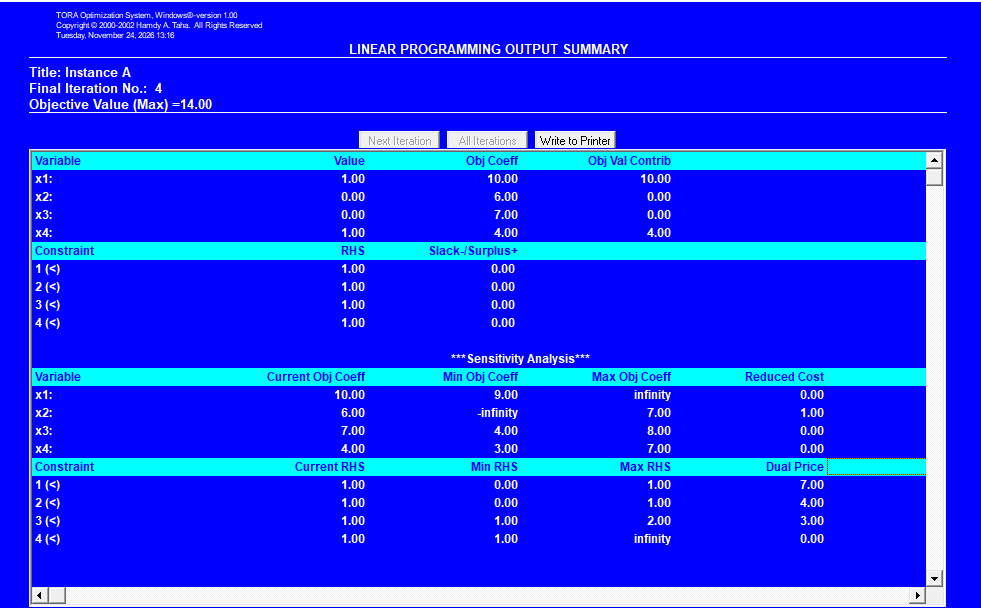
\includegraphics[width=\linewidth]{figures/tora-A-primal.png}\\{\scriptsize (a) assignment LP of $A$, with sensitivity}
\end{minipage}\hfill
\begin{minipage}[t]{0.32\textwidth}\centering
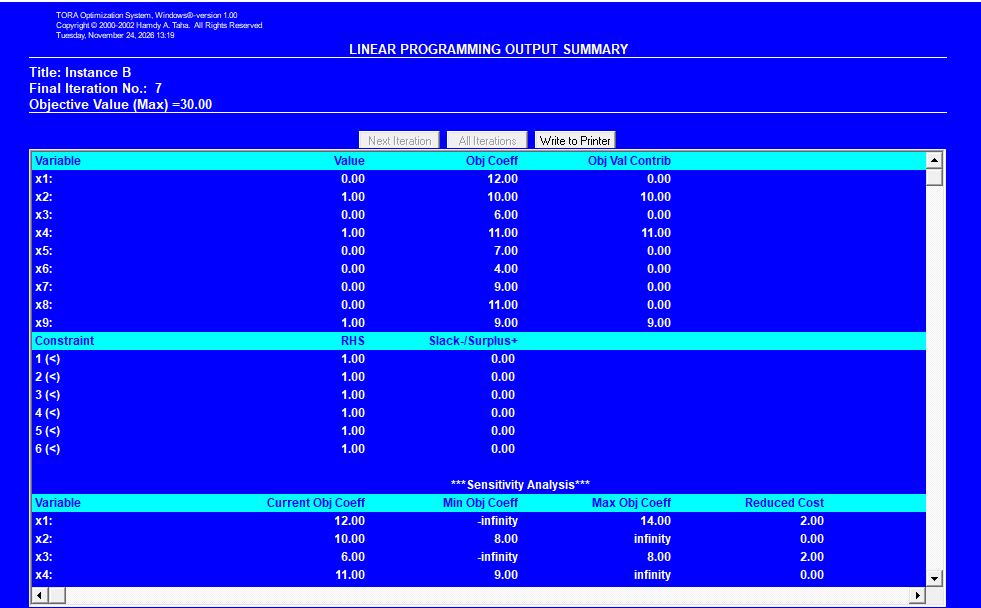
\includegraphics[width=\linewidth]{figures/tora-B-primal.png}\\{\scriptsize (b) assignment LP of $B$}
\end{minipage}\hfill
\begin{minipage}[t]{0.32\textwidth}\centering
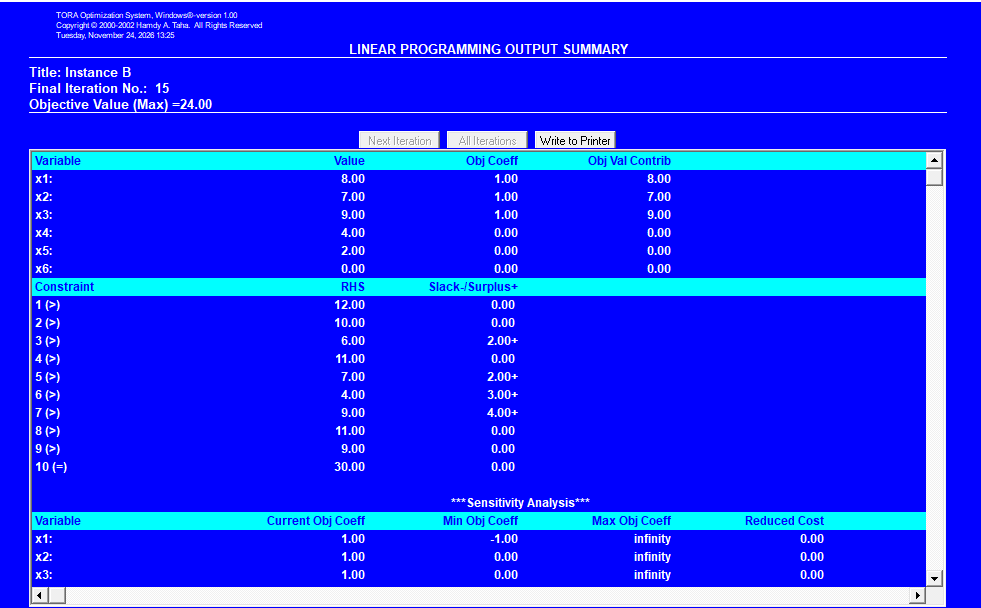
\includegraphics[width=\linewidth]{figures/tora-B-RO.png}\\{\scriptsize (c) RO LP of $B$, M-method}
\end{minipage}

\vspace{0.5em}
\begin{minipage}[t]{0.32\textwidth}\centering
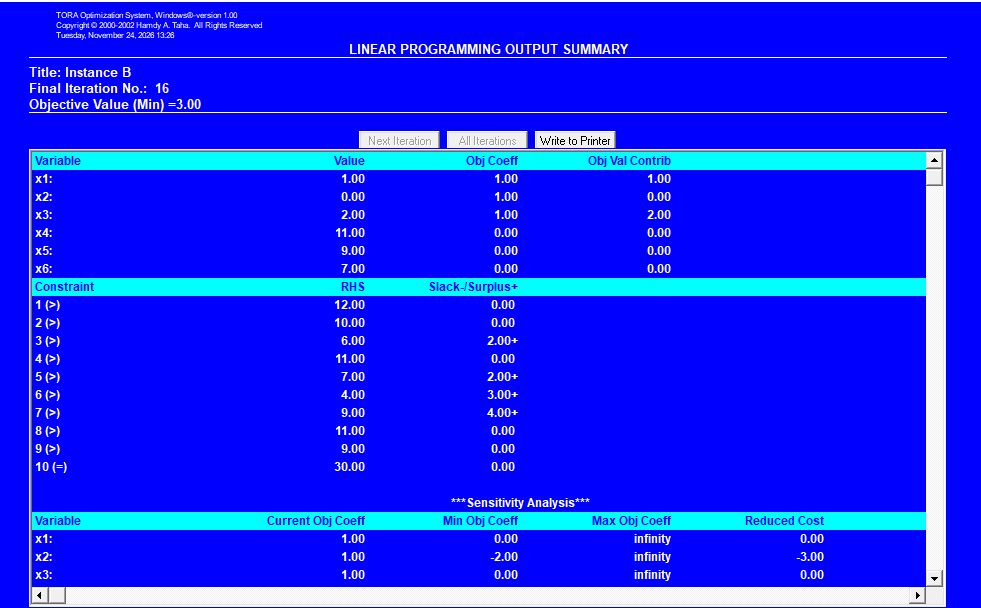
\includegraphics[width=\linewidth]{figures/tora-B-DO.png}\\{\scriptsize (d) DO LP of $B$, M-method}
\end{minipage}\hfill
\begin{minipage}[t]{0.32\textwidth}\centering
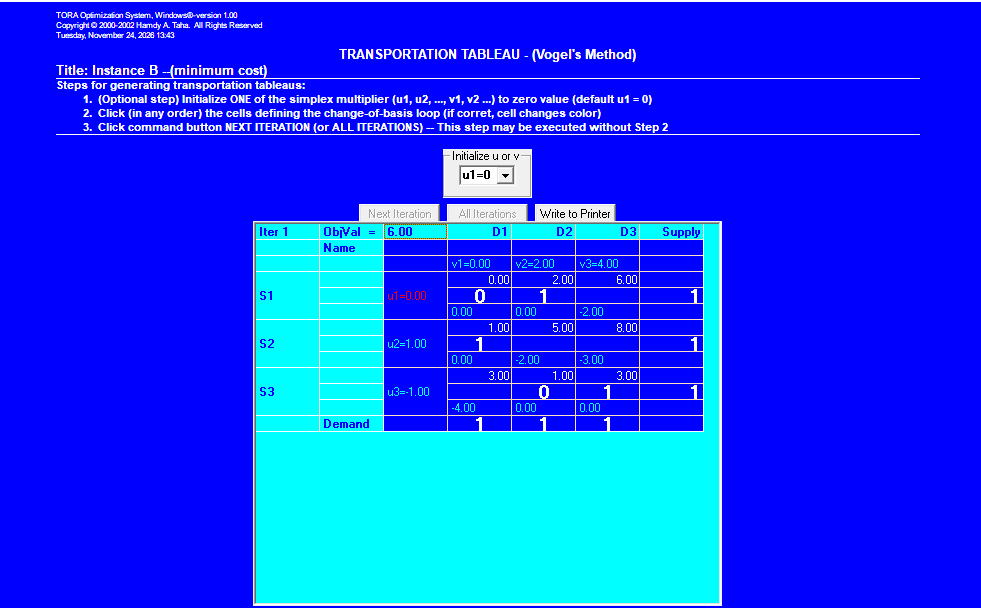
\includegraphics[width=\linewidth]{figures/tora-B-transport-Vogel.png}\\{\scriptsize (e) transportation model of $B$, Vogel start}
\end{minipage}\hfill
\begin{minipage}[t]{0.32\textwidth}\centering
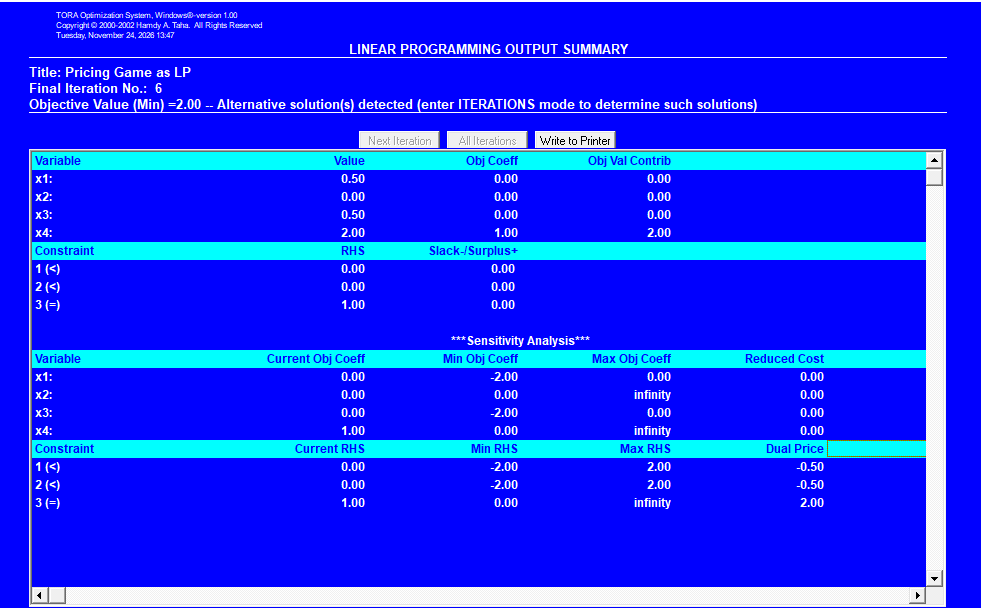
\includegraphics[width=\linewidth]{figures/tora-game-LP.png}\\{\scriptsize (f) pricing game as an LP}
\end{minipage}
\caption{TORA output for the models in Table~\ref{tab:tora}.}
\label{fig:tora}
\end{figure}

\textbf{What the code adds.} TORA cannot repeat thousands of noisy solves or try every misreport, so those run in our code: a small JavaScript program with 37 tests and a script that recomputes every number in this report. The same code runs as an interactive web page (Figure~\ref{fig:page}). The user enters a surplus table of up to four riders and four drivers, or picks $A$ or $B$. The page shows the matching, each pair's split with a slider from RO through MID to DO, the price ranges, the error study, the misreport table and the game, and recomputes all of it when a number changes.

\begin{figure}[htbp]
\centering
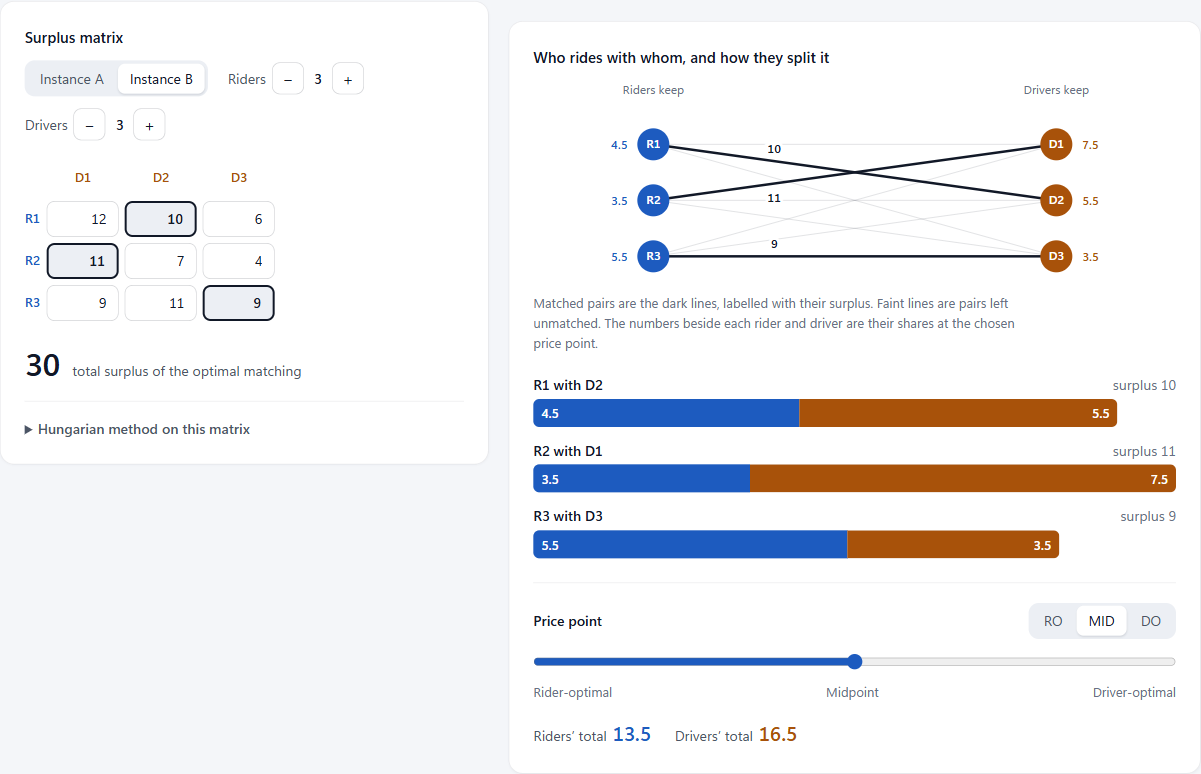
\includegraphics[width=0.78\textwidth]{figures/page-market.png}
\caption{The interactive page on $B$ at MID: the editable surplus table with the matching outlined (left), and the matching, each pair's split and the price-point slider (right).}
\label{fig:page}
\end{figure}

\section{Selected Progress: What the Experiments Show}

All numbers below come from our code, with a fixed random seed and 4000 random draws per value of $\sigma$.

\subsection{Prediction error}

Each draw adds error to $B$, solves the predicted market, and compares it with the true one. We record whether the matching changed, how much true surplus the predicted matching loses, how far each price point moved (the total absolute change of the six shares), and whether any true pair would block the predicted prices (Table~\ref{tab:noise}, Figure~\ref{fig:noise}).

\begin{table}[h]
\centering\small
\begin{tabular}{lcccccc}
\toprule
$\sigma$ & P(matching changes) & Mean surplus lost & \multicolumn{3}{c}{Mean price shift} & P(some pair blocks) \\
 & & & RO & MID & DO & MID \\
\midrule
0.25 & 0.000 & 0.000 & 1.66 & 1.34 & 1.67 & 0.967 \\
0.5  & 0.047 & 0.100 & 3.26 & 2.61 & 3.18 & 0.967 \\
1    & 0.297 & 0.651 & 5.63 & 4.39 & 5.02 & 0.954 \\
2    & 0.537 & 1.278 & 9.15 & 6.82 & 7.73 & 0.885 \\
\bottomrule
\end{tabular}
\caption{Prediction error on $B$ ($V=30$). With $\sigma=0$ every entry is 0.}
\label{tab:noise}
\end{table}

\begin{figure}[h]
\centering
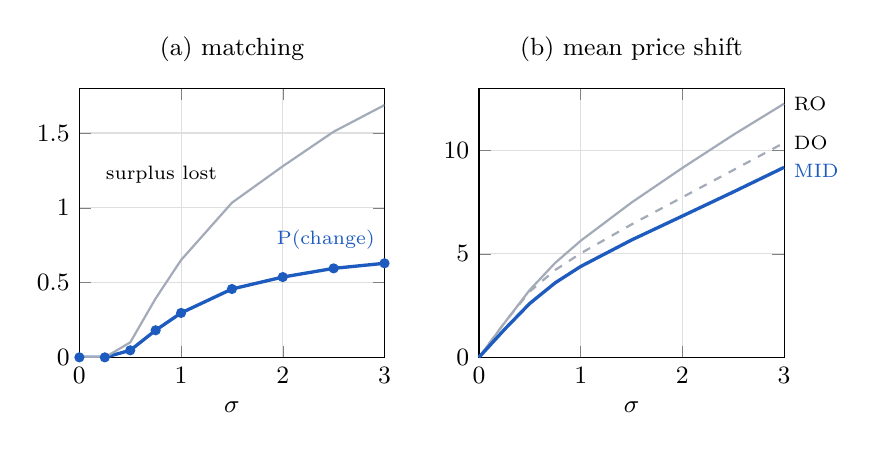
\begin{tikzpicture}
\begin{axis}[
  name=left, width=0.45\textwidth, height=5cm,
  xmin=0, xmax=3, ymin=0, ymax=1.8,
  xlabel={$\sigma$}, grid=major, grid style={gray!25},
  tick label style={font=\small}, label style={font=\small},
  title={\small (a) matching}]
\addplot[very thick, rider, mark=*, mark size=1.2pt] coordinates {(0,0) (0.25,0) (0.5,0.047) (0.75,0.181) (1,0.297) (1.5,0.457) (2,0.537) (2.5,0.595) (3,0.629)};
\node[font=\scriptsize, anchor=south east, text=rider] at (axis cs:3,0.66) {P(change)};
\addplot[thick, quiet] coordinates {(0,0) (0.25,0) (0.5,0.100) (0.75,0.394) (1,0.651) (1.5,1.034) (2,1.278) (2.5,1.509) (3,1.687)};
\node[font=\scriptsize, anchor=south east] at (axis cs:1.45,1.1) {surplus lost};
\end{axis}
\begin{axis}[
  at={(left.east)}, anchor=west, xshift=1.2cm,
  width=0.45\textwidth, height=5cm, clip=false,
  xmin=0, xmax=3, ymin=0, ymax=13,
  xlabel={$\sigma$}, grid=major, grid style={gray!25},
  tick label style={font=\small}, label style={font=\small},
  title={\small (b) mean price shift}]
\addplot[thick, quiet] coordinates {(0,0) (0.25,1.658) (0.5,3.261) (0.75,4.565) (1,5.630) (1.5,7.476) (2,9.147) (2.5,10.744) (3,12.251)};
\addplot[thick, quiet, dashed] coordinates {(0,0) (0.25,1.673) (0.5,3.183) (0.75,4.221) (1,5.022) (1.5,6.420) (2,7.731) (2.5,9.042) (3,10.361)};
\addplot[very thick, rider] coordinates {(0,0) (0.25,1.343) (0.5,2.606) (0.75,3.602) (1,4.389) (1.5,5.668) (2,6.825) (2.5,7.987) (3,9.176)};
\node[font=\scriptsize, anchor=west] at (axis cs:3,12.25) {RO};
\node[font=\scriptsize, anchor=west] at (axis cs:3,10.36) {DO};
\node[font=\scriptsize, anchor=west, text=rider] at (axis cs:3,9.0) {MID};
\end{axis}
\end{tikzpicture}
\caption{$B$ under prediction error. (a) How often the predicted matching differs from the true one, and the mean surplus lost. (b) How far each price point moves.}
\label{fig:noise}
\end{figure}

\begin{itemize}
  \item The matching survives small errors. The second-best matching is 2 units behind, so at $\sigma=0.25$ it never changes. At $\sigma=1$ it changes in 30\% of draws, but only 0.65 of the 30 units (2\%) are lost, because the wrong matching is almost as good.
  \item Prices move far more than the surplus. At $\sigma=1$ the six shares move by 4.4 to 5.6 in total, seven to nine times the surplus lost. MID moves least at every $\sigma$.
  \item Prices computed from predictions are almost never exactly stable for the true values: for $\sigma\le2$, in at least 88\% of draws some true pair would block, usually by a small amount. Several core constraints hold with equality, so any error pushes one of them the wrong way.
\end{itemize}

\subsection{Misreporting}

One rider changes their own row of the table, or one driver their own column, by $-2$, $-1$, $+1$ or $+2$. The platform solves the reported table and prices it at RO, MID or DO. The gain is what that person really earns (true surplus with their new partner minus the partner's share) minus what they earn by telling the truth. That gives 24 cases per price point (Table~\ref{tab:manip}).

\begin{table}[h]
\centering\small
\begin{tabular}{lccc}
\toprule
Price point & Best rider gain & Best driver gain & Cases with a gain \\
\midrule
RO  & 0 & 2 & 2 of 24 \\
MID & 1 & 1 & 5 of 24 \\
DO  & 2 & 0 & 3 of 24 \\
\bottomrule
\end{tabular}
\caption{Best gain from one false report in $B$.}
\label{tab:manip}
\end{table}

RO pays each rider their marginal contribution, so no rider can gain by lying under RO; DO does the same for drivers. This is a known result~\cite{leonard,dgs}, and our check on 200 random $4\times4$ markets found no gain larger than 0. The protection covers only one side: under RO, driver D3 gains 2 by understating by 2, and under DO, rider R2 gains 2 the same way. Every profitable lie we found was an understatement. MID limits the best gain to 1 on both sides.

\subsection{Which price should the platform choose?}

We model the choice as a zero-sum game. The platform picks RO, MID or DO; a manipulator picks which side to act on; the payoff is the best gain from Table~\ref{tab:manip}, which the platform wants small:
\[
M=\begin{array}{c|cc}
 & \text{riders} & \text{drivers}\\\hline
\text{RO} & 0 & 2\\
\text{MID} & 1 & 1\\
\text{DO} & 2 & 0
\end{array}
\qquad
\min_i\max_j m_{ij}=1,\quad \max_j\min_i m_{ij}=0 .
\]
The two differ, so there is no saddle point and the players mix. If the manipulator targets riders with probability $y$, the three rows give expected gains $2-2y$, $1$ and $2y$. The platform takes the lowest line at every $y$; the manipulator takes the highest point of that lower envelope, at $y=\tfrac12$ with value 1 (Figure~\ref{fig:game}). The value of the game is 1. The manipulator splits half and half, and the platform is optimal with pure MID or with half RO and half DO. As an LP (each payoff raised by 1 so that TORA's variables stay non-negative): minimise $w$ subject to $p_1+2p_2+3p_3\le w$, $3p_1+2p_2+p_3\le w$, $p_1+p_2+p_3=1$, which gives $w=2$ and value 1. The solver also reproduces the textbook game $\begin{pmatrix}3&-1\\-2&4\end{pmatrix}$: value 1, row mix $(0.6,0.4)$, column mix $(0.5,0.5)$.

\begin{figure}[h]
\centering
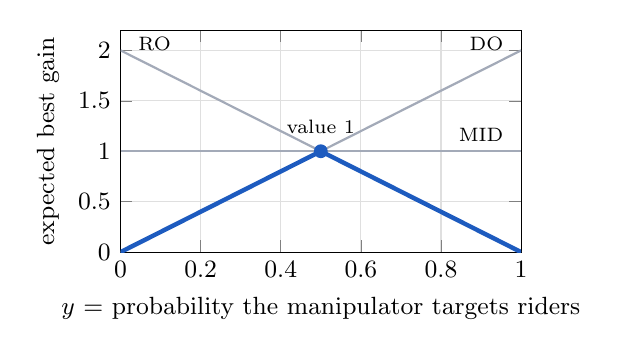
\begin{tikzpicture}
\begin{axis}[
  width=0.55\textwidth, height=4.4cm,
  xmin=0, xmax=1, ymin=0, ymax=2.2,
  xlabel={$y$ = probability the manipulator targets riders}, ylabel={expected best gain},
  grid=major, grid style={gray!25}, tick label style={font=\small}, label style={font=\small}]
\addplot[thick, quiet, domain=0:1] {2-2*x};
\addplot[thick, quiet, domain=0:1] {1};
\addplot[thick, quiet, domain=0:1] {2*x};
\addplot[ultra thick, rider] coordinates {(0,0) (0.5,1) (1,0)};
\fill[rider] (axis cs:0.5,1) circle (2.5pt);
\node[font=\scriptsize, anchor=south west] at (axis cs:0.02,1.9) {RO};
\node[font=\scriptsize, anchor=south east] at (axis cs:0.98,1.9) {DO};
\node[font=\scriptsize, anchor=south east] at (axis cs:0.98,1.0) {MID};
\node[font=\scriptsize, anchor=south] at (axis cs:0.5,1.08) {value 1};
\end{axis}
\end{tikzpicture}
\caption{Graphical method for the pricing game. The thick blue line is the platform's lower envelope; its highest point is the value of the game.}
\label{fig:game}
\end{figure}

\textbf{Conclusion.} The matching tolerates prediction error well; the prices do not, and MID is the most stable of the three. RO and DO each protect one side against lying and leave the other side open, while MID limits both sides to a gain of 1 and is optimal in the game. On this market the platform should price at MID, and use RO or DO only when it knows which side might misreport.

\textbf{Limits.} The error and game results use one $3\times3$ market. Misreports are single people shifting by up to 2, errors are independent and normal, and the predictor is simulated, not fitted to real trip data.

{\footnotesize
\begin{thebibliography}{9}
\setlength{\itemsep}{0pt}
\bibitem{shapley} L. S. Shapley and M. Shubik. The assignment game I: The core. \emph{International Journal of Game Theory}, 1:111--130, 1971.
\bibitem{leonard} H. B. Leonard. Elicitation of honest preferences for the assignment of individuals to positions. \emph{Journal of Political Economy}, 91(3):461--479, 1983.
\bibitem{dgs} G. Demange, D. Gale and M. Sotomayor. Multi-item auctions. \emph{Journal of Political Economy}, 94(4):863--872, 1986.
\bibitem{taha} H. A. Taha. \emph{Operations Research: An Introduction}. Pearson, 10th edition, 2017.
\end{thebibliography}
}

\section*{Project Repository}
{\small Code: \texttt{github.com/Anirudh2007/core-pricing} \quad Page: \texttt{anirudh2007.github.io/core-pricing}}

\end{document}
